\documentclass[a4paper,12pt]{article}
\usepackage{geometry}
\usepackage{graphicx}
\usepackage{amsmath}
\usepackage{amsfonts}
\usepackage{hyperref}
\usepackage{titlesec}

% Page settings
\geometry{top=2cm,bottom=2cm,left=2cm,right=2cm}
\titleformat{\section}{\large\bfseries}{\thesection}{1em}{}
\titleformat{\subsection}{\bfseries}{\thesubsection}{1em}{}

\begin{document}

\begin{titlepage}
    \centering
    {\scshape\LARGE UNIVERSITY OF SCIENCE AND TECHNOLOGY OF HANOI\par}
    \vspace{1cm}
    {\scshape\Large Information and Communication Technology Department\par}
    \vspace{2cm}
    {\huge\bfseries DISTRIBUTED SYSTEMS\par}
    \vspace{0.5cm}
    {\huge\bfseries REPORT - FTP Proxy via RPC\par}
    \vfill
    \begin{flushright}
        Nguyen Ha Trung - 22BI13436\\
        Nguyen Quang Bach - 22BI13053\\
        Do Le Hoang Viet - 22BI13463\\
        Le Quang Tung - 22BI13454\\
        Nguyen Quang Minh - 22BI13299\\
        Pham Le Vu - 22BI13480\\
        Tran Duc Trung - BA12-179
    \end{flushright}
    \vfill
    {\large HANOI, DEC 2024\par}
\end{titlepage}

\section{Abstract}
This system, called "FTP over RPC," shows how we can use FTP (File Transfer Protocol) with RPC (Remote Procedure Call). The main goal is to make an FTP proxy that uses RPC to handle all the file transfers. Doing this makes the process safer, easier to manage, and better at fixing errors.

\section{Introduction}
\subsection{What Are FTP and RPC?}
FTP is a way to send files between a client (you) and a server. It’s old and works fine but has issues like being unsafe and not great for big systems. RPC lets one computer ask another to do something, almost like they’re working together on the same machine. It makes networking stuff easier to deal with.

\subsection{Why Use FTP with RPC?}
Switching FTP to work with RPC helps because:
\begin{itemize}
    \item It fixes FTP’s security issues.
    \item It works better in complicated systems.
    \item It’s easier to handle errors.
\end{itemize}

\subsection{What’s an FTP Proxy?}
An FTP proxy is like a middleman. The client asks it to do something, and it talks to the server to make it happen. This makes the whole process smoother and easier to control.

\section{Background}
\subsection{How FTP Works}
FTP uses two connections:
\begin{itemize}
    \item One for sending commands like upload or download.
    \item One for sending or receiving the actual files.
\end{itemize}

\subsection{How RPC Works}
RPC lets one computer call a function on another computer, like:
\begin{itemize}
    \item The client asks the server to do something.
    \item The server does it and sends back the result.
\end{itemize}

\subsection{Why FTP Needs Help}
FTP isn’t safe—it doesn’t hide your data or password and struggles in big, modern systems.

\section{System Architecture}
\subsection{How the System Is Set Up}
The "FTP over RPC" system has three parts:
\begin{itemize}
    \item Client: This sends requests to upload, download, or list files.
    \item Server: This does the actual work, like saving or sending files.
    \item Proxy: This connects the client and server using RPC.
\end{itemize}

\subsection{Why Use RPC?}
RPC makes everything easier by hiding the complicated network details.
\begin{figure}[h]
    \centering
    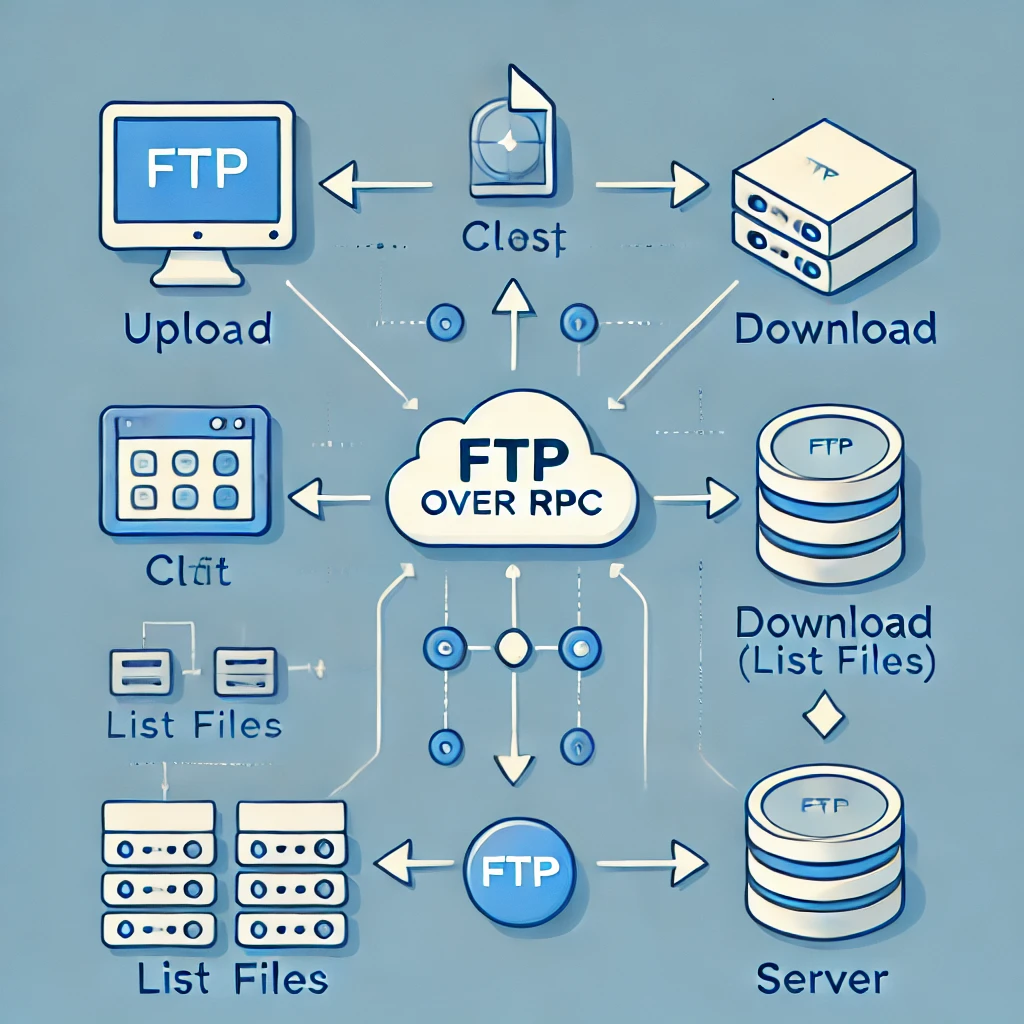
\includegraphics[width=0.8\textwidth]{1.png} 
    \caption{Architecture Diagram of FTP over RPC}
\end{figure}
\section{Design Analysis}
\subsection{How It Works}
The client sends a request, like "upload this file." The server does what it’s asked and sends back a reply.

\subsection{What Happens When Something Goes Wrong?}
If there’s a problem (like a missing file), the server sends an error message. If the server doesn’t answer, the system stops waiting after a while.

\subsection{How It Stays Safe}
Data is encrypted while it’s being sent. Only verified clients are allowed to send requests.

\section{Implementation}
\subsection{What Tools Are Used?}
The code is written in C. A tool called rpcgen is used to create RPC code automatically.

\subsection{What Can It Do?}
\begin{itemize}
    \item upload: Send a file to the server.
    \item download: Get a file from the server.
    \item list\_files: See all the files on the server.
\end{itemize}

\subsection{Example Code: Upload Function}
\begin{verbatim}
int *upload_1_svc(char **file_name, struct svc_req *req) {  
    static int result = 0;  
    FILE *file = fopen(*file_name, "wb");  
    if (!file) {  
        result = -1;  
        return &result;  
    }  
    fwrite((*file_name), sizeof(char), strlen(*file_name), file);  
    fclose(file);  
    result = 0;  
    return &result;  
}
\end{verbatim}

\section{Results and Testing}
\subsection{How Well Does It Work?}
Small files (less than 10MB): Very fast.\\
Big files (more than 100MB): Slower because it depends on your internet speed.

\subsection{What Did We Test?}
\begin{itemize}
    \item File transfers: Uploaded and downloaded files like .txt and .jpg.
    \item File listings: Showed the correct list of files on the server.
    \item Errors: Responded properly when files were missing or something went wrong.
\end{itemize}

\section{Comparison with Other Solutions}
This system is better than normal FTP because:
\begin{figure}[h]
    \centering
    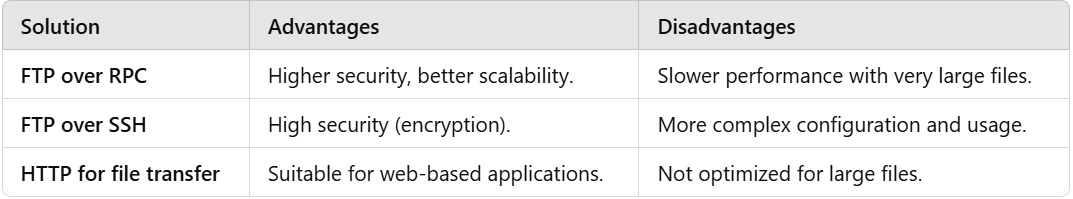
\includegraphics[width=0.8\textwidth]{2.png} 
    \caption{}
\end{figure}
\begin{itemize}
    \item It’s safer.
    \item It works well in big, complex networks.
    \item It’s better at handling errors.
\end{itemize}

\section{Practical Applications}
\begin{itemize}
    \item File Management Companies: Storing and transferring files between branches.
    \item Education Sector: Sharing learning materials across remote locations.
\end{itemize}

\section{Conclusion}
The "FTP over RPC" system fixes many of FTP’s problems by using RPC. It’s safer, easier to use, and works better for today’s networks. There’s still room to improve, like adding stronger encryption and speeding up transfers for big files.

\section{References}
\begin{itemize}
    \item Andrew S. Tanenbaum, {\itshape Distributed Systems: Principles and Paradigms}
    \item RFC 959 - File Transfer Protocol Specification
    \item Linux Documentation on RPC Programming
\end{itemize}

\end{document}